\section{Propagazione guidata}
Le equazioni delle onde piane uniformi trovate sinora si possono quindi applicare anche per la propagazione di onde elettromagnetiche in conduttori, per esempio
\begin{description}
	\item \textbf{linee bifilari} come il doppino telefonico

	Le linee di forza del campo elettrico nella linea bifilare sono simili a quelle di un condensatore, ossia in ogni punto $\E\perp\H\perp\k$.

	\item \textbf{linee coassiali}, come il cavo dell'antenna televisiva

	In questo caso le linee di campo sono analoghe a quelle di un condensatore cilindrico: il campo elettrico è ortogonale alla circonferenza, mentre quello magnetico sono parallele ad essa.

	\item \textbf{guide rettangolari} impiegate nella trasmissione ad alta potenza

	\item \textbf{linee a microstriscia} utilizzate per trasportare segnali in circuiti stampati
\end{description}
Accenniamo ora come si propaga l'onda in alcune di queste guide, poiché il segnale di norma andrà trasportato all'antenna dal generatore.

\paragraph{Impedenza caratteristica}
Cerchiamo ora di valutare l'impedenza caratteristica della linea e, in particolare, come sfruttarla per ridurre al minimo le perdite.

La tensione e la corrente nella linea coassiale si possono scrivere come
\begin{esp}
	V&= \int_{r_{int}}^{r_{ext}} \E \cdot \de \vec{l} \\
	I&= \oint \H \cdot \de \vec{l} \\
	\implies Z_C &= \frac{V_o}{I_o} \text{ impedenza caratteristica della linea}
\end{esp}
Definendo inoltre
\begin{itemize}
	\item $l$ l'induttanza per unità di lunghezza $\frac{H}{m}$
	\item $c$ la capacità per unità di lunghezza $\frac{F}{m}$
\end{itemize}
si ottiene che l'impedenza caratteristica risulta
\begin{equation}
	Z_C = \sqrt{\frac{l}{c}} = F \cdot \sqrt{\frac{\mu}{\epsilon}}
\end{equation}
dove $F$ è detto \emph{fattore di forma}.

Possiamo quindi riscrivere le equazioni per la tensione e la corrente nel cavo coassiale come
\begin{esp}
	V(z) &= V_o \cdot e^{-\jmath \beta \cdot z}\\
	I(z) &= I_o \cdot e^{-\jmath \beta \cdot z}
\end{esp}

\chapter{Antenne}
In questo capitolo analizzeremo le antenne, partendo inizialmente con i potenziali elettromagnetici e cercando di riformulare le equazioni di Maxwell affinché siano più semplici da risolvere nei casi che analizzeremo.

Vedremo quindi l'equazione di Helmoltz e la scelta di Lorentz. Inizieremo quindi a studiare le antenne partendo dal caso del dipolo elementare, ideale e non realizzabile nella realtà, ma utile per fare le prime approssimazioni. Estenderemo quindi il dipolo elementare al dipolo corto per studiare poi le antenne lineari, le schiere e le patch.

Riprendiamo le equazioni di Maxwell scritte con i vettori di Steinmetz.
\begin{equation}\label{eq:maxw-ant}\begin{cases}
	\rot\E = -\jmath \omega \mu\H(\r) \textcolor[rgb]{0.8,0,0}{+ \M} \\
	\rot\H = \jmath \omega \epsilon \E + \J\\
	\diverg\H=0\\
	\diverg \E = \frac{\rho}{\epsilon}
\end{cases}\end{equation}
Ora aggiungiamo un termine $\M$ fittizio di correnti \emph{magnetiche}, affinché le equazioni risultino simmetriche e si possa scrivere, in seguito, il sistema di sorgenti equivalenti.

\subsubsection{Potenziali elettromagnetici}
Definiamo quindi $\A$ \emph{potenziale vettore magnetico} il campo per cui $\H = \frac{1}{\mu} \cdot \rot \A$.

\begin{theorem}[Teorema di Helmoltz]
	Un campo vettoriale $\A$ è univocamente definito se sono fissati $\rot \A$ e $\diverg \A$.
\end{theorem}

Per definire propriamente il potenziale $\A$, dobbiamo dunque fornire l'espressione per la $\diverg \A$.
\begin{esp} \label{eq:AE}
	\rot\E &= - \jmath \omega \cdot \mu \frac{1}{\mu} \rot \A \quad \Leftrightarrow \quad \rot\left(\rot \E + \jmath \omega \A\right)=0
\end{esp}

Questo ci permette di affermare che il termine tra parentesi in \autoref{eq:AE} deve essere \emph{costante} a meno di un termine che si annulli con l'operazione di rotore.

Data una funzione $\phi$ scalare, sappiamo che $ \rot(\nabla \phi)=0$: una funzione così costruita risulta perciò una buona candidata per scrivere

\begin{esp}
	\E +& \jmath \omega \A = -\nabla\phi \quad \implies \E = -\jmath \omega \A - \nabla \phi \\
\end{esp}

Dal punto di vista dimensionale, $\phi$ si misura in $V$, perciò viene chiamata \emph{potenziale scalare elettrico}.

\smallbreak
Analizziamo ora la seconda equazione di Maxwell.
\begin{esp}
	\rot \H &= \jmath \omega \epsilon_c \cdot \E + \J = \mu \cdot \rot\left(\frac{1}{\mu} \rot \A\right)\\
	\rot \H &= \jmath \omega \mu \epsilon_c \cdot \left(-\jmath \omega \A - \nabla \phi \right) + \J \mu \\
	-\nabla^2\A + \diverg(\nabla \A) &= \omega^2 \mu \epsilon_c \A - \jmath \omega \mu \epsilon_c \nabla \phi + \mu \J \\
	\nabla^2 \A + \omega^2 \mu \epsilon_c \A
		&= -\mu\J + \diverg(\nabla\A) + \jmath \omega \mu \epsilon_c \nabla \phi \\
	\underbrace{-\nabla^2\A + \diverg(\nabla \A)}_{(1)} &=\underbrace{-\mu\J}_{(2)} + \diverg\left(\underbrace{\nabla \A + \jmath \omega \mu \epsilon_c \phi}_{(3)}\right)\\
\end{esp}

Riconosciamo nel termine (1) il primo membro caratteristico dell'equazione delle onde tridimensionale, in (2) il contributo di termine noto delle sorgenti.

IL termine (3) risulta fuori posto, ma seguendo esso può essere reso nullo, come mostrato in seguito.

\paragraph{Scelta di Lorentz}
Poiché abbiamo ancora un grado di libertà per definire $\A$, secondo il teorema di Helmotz, possiamo scegliere
\begin{equation}
	\diverg \A = -\jmath \omega \mu \epsilon_c \phi
\end{equation}
Otteniamo quindi l'\emph{equazione di Helmoltz non omogenea}.
\begin{equation}
	\nabla^2\A + \omega^2 \mu\epsilon_c\A =-\mu \J
\end{equation}
Dobbiamo ora determinare il valore di $\phi$, cosa che faremo sfruttando la terza legge di Maxwell.
\begin{esp*}
	\diverg\E
		= \frac{\rho}{\epsilon} ~~ \implies ~~ &
		\diverg\left(-\jmath \omega \A - \nabla \phi	 \right)= \frac{\rho}{\epsilon}\\
	 & \jmath \omega \A + \nabla \phi= -\frac{\rho}{\epsilon}	 \\
	&\jmath\omega\left(-\jmath \omega\mu\epsilon_c\phi\right) + \nabla^2\phi = - \frac{\rho}{\epsilon}\\
\end{esp*}

Otteniamo così l'equazione \emph{scalare} di Helmoltz non omogenea.
\begin{esp*}
	&\omega^2\mu\epsilon_c\phi + \nabla^2 \phi = -\frac{\rho}{\epsilon}
\end{esp*}

Riassumendo, le equazioni di Maxwell si possono riscrivere nella forma delle equazioni di Helmotz: adotteremo queste ultime per descrivere l'elettromagnetismo, per la maggiore facilità di risoluzione nello studio delle antenne.

\begin{esp}\label{eq:helmolts-lorentz}
	\begin{dcases}
		~ \nabla^2\A + \omega^2\mu\epsilon_c\A = -\mu\J \\
		~ \nabla^2\phi + \omega^2\mu\epsilon_c\phi = -\frac{\rho}{\epsilon}
	\end{dcases}
\end{esp}

\section{Dipolo elementare}
Si può notare che le equazioni di Helmoltz trovate sono lineari: il principio di sovrapposizione degli effetti ci consente perciò di estendere a casi complessi lo studio di sorgenti semplici.

Partiamo perciò analizzando l'azione del \emph{dipolo elementare}, un'antenna filiforme di lunghezza infinitesima $\Delta z$.

La sua distribuzione di corrente si può scrivere perciò come
\begin{esp} \label{eq:dipolo_elementare}
	\J &= I \, \delta(x)\delta(y) g(z) \hhat{z} \\
	\text{dove } g(z) &= \begin{cases}
		1 & - \frac{\Delta z}{2} \le z \le \frac{\Delta z}{2} \\
		0 & \text{altrove}
	\end{cases}
\end{esp}

Risolviamo quindi l'equazione \autoref{eq:helmolts-lorentz} di Helmoltz non omogenea per questa distribuzione delle sorgenti.
\begin{esp*}
	\begin{cases}
		\nabla^2 A_{x,y} + \omega^2 \mu\epsilon_c A_{x,y} =0 \\
		\nabla^2 A_{z} + \omega^2 \mu\epsilon_c A_{z} =-\mu J_z
	\end{cases}
\end{esp*}

Osservando la prima equazione, possiamo subito notare che $A_x = A_y = 0$ è una soluzione valida: per questo motivo la adotteremo e procederemo a valutare $A_z$.

Ci focalizziamo ora sulla \emph{propagazione} dell'onda elettromagnetica, ponendo $\r \neq 0$: questa scelta ci permette di rendere nullo il termine noto della seconda equazione nella regione di spazio considerata.

\begin{esp}
	\forall \r \neq 0, ~ \nabla^2 A_{z} + \omega^2 \mu\epsilon_c A_{z} = 0
\end{esp}

\smallbreak
Supponiamo ora che il materiale sia un perfetto isolante, perciò $\sigma=0$ e $\epsilon_c = \epsilon \in \R$.

\begin{equation} \label{eq:helmotz_vuoto}
	\nabla^2 A_{z} + \omega^2 \mu\epsilon A_{z} =0
\end{equation}

Procediamo ora con un'ipotesi di soluzione: supponiamo che il potenziale vettore lungo l'asse $z$ abbia l'andamento di un'onda sferica.
\begin{esp*}
	&A_z(r,\theta,\phi) =A_z(r) = \frac{f(r)}{r} \\
\end{esp*}

Sostituendo l'espressione in \autoref{eq:helmotz_vuoto}, si ottiene perciò
\begin{esp*}
	\nabla^2 A_z
	& = \frac{1}{r^2} \deriv{}{r}\left(r^2 \deriv{A_z(r)}{r}\right) \\
	& = \frac{1}{r^2} \deriv{}{r}\left(r^2 \deriv{\frac{f(r)}{r}}{r}\right) + \omega^2 \mu\epsilon\frac{f(r)}{r} \\
	& = \frac{1}{r} \deriv{}{r}\left(r^2 \deriv{\frac{f'(r)\cdot r - f}{r^2}}{r}\right) + \omega^2 \mu\epsilon\frac{f(r)}{r}\\
	& = \frac{1}{r} \left[
		f^{\prime\prime}(r)\cdot r + f^\prime(r)\cdot 1 - f^\prime(r) \right]
	+ \omega^2\mu\epsilon f(r) = 0\\
\end{esp*}
dove $f^\prime(r) = \deriv{f(r)}{r}$ e $f^{\prime\prime}(r) =\deriv[2]{f(r)}{r}$.

\smallbreak
Concludiamo quindi che
\begin{equation*}
	f^{\prime\prime}(r) + \omega^2\mu\epsilon f(r) = 0
\end{equation*}

e perciò, risolvendo l'equazione differenziale,
\begin{equation}
	f(r) = c \, e^{-\jmath \beta r} + d \, e^{\jmath \beta r}
\end{equation}
con $c,d \in \C$ costanti di integrazione, $\beta = \omega\sqrt{\mu\epsilon}$.

$A_z(r)$ risulta quindi essere
\begin{equation}
	A_z(r) = \frac{c}{r}\, \ejbr +\frac{d}{r}\, \ejbrp
\end{equation}
che non è più un'onda piana, essendo gli esponenziali \emph{smorzati} in $r$.

Inoltre le due componenti progressiva e regressiva dell'onda sono di tipo sferico, infatti $A_z$, e quindi $\A$, non dipende da $\theta$ e $\phi$, ma solamente da $r$.
\begin{itemize}
	\item $|A_z| = \left|\frac{c}{r}\right|$
	~ la superficie equiampiezza è una sfera di raggio r
	\item $\measuredangle A_z = \beta r$
	~ la superficie equifase è una sfera di raggio r
\end{itemize}

\smallbreak
La soluzione generale trovata in precedenza è però incompleta: se da una parte è possibile impostare $d = 0$ ipotizzando l'assenza di riflessioni, è tuttora necessario stabilire $c$ dalle condizioni al contorno, \emph{estendendo} la soluzione per $\r = 0$.

Integrando l'equazione di Helmotz non omogenea nel volume della sfera di di raggio $\r_0$ centrata nell'origine, otteniamo
\begin{esp*}
	\int_V \nabla^2 A_z \de V + \omega^2 \mu \epsilon \int_V A_z \de V &= -\mu \int_V J_z \de V \\
	\int_V \diverg(\nabla A_z) \de V + \omega^2 \mu \epsilon \int_V A_z \de V &= -\mu \int_V I \delta(x)\delta(y) g(z) \de V
\end{esp*}
dove $g(z)$, definita in \autoref{eq:dipolo_elementare}, è la di--stribuzione di corrente del dipolo.

Applicando il teorema della divergenza al primo membro otteniamo che
\begin{esp} \label{eq:helmotz_dipolo_el}
	\int_{S_V} \nabla A_z \hhat{n} \de S
	+ \omega^2 \mu \epsilon \int_V A_z \de V
	= -\mu \int_V I \delta(x)\delta(y) F(z) \de V \\
\end{esp}

Da quanto ricavato nella risoluzione dell'equazione di Helmotz omogenea, sappiamo che nella superficie $S_V$ vale
\begin{esp*}
	\nabla A_z \cdot \hhat{n}
	= \frac{\de}{\de r} A_z \hhat{r} \cdot \hat{n}
	\stackrel{(*)}{=} c \left(
			-\jmath \beta \frac{\ejbr}{r}
			- \frac{\ejbrp}{r^2}
		\right)
\end{esp*}
dove in (*) il prodotto scalare tra versori è 1, perché la normale in ogni punto della sfera è parallela al raggio che lo individua.

Sostituendo il risultato appena ottenuto a \autoref{eq:helmotz_dipolo_el} cerchiamo ora la continuità nell'origine, prendendone il limite per $r \to 0$.

% nota che nella formula mi è toccato usare \bigg[ invece di \left[ \right] perché altrimenti non poteva starci dentro & per lo split
\begin{esp*}
	\lim_{r^\prime \to 0} \bigg[ \int_{S_V} c & \left(
		-\jmath \beta \frac{\ejbr}{r}
		- \frac{\ejbrp}{r^2} \right) \de S
	+ \omega^2 \mu \epsilon \int_V \left(\frac{c}{r}\cdot \ejbr \right) \de V \bigg] = \\
	& = -\mu \lim_{r^\prime \to 0} \int_V I \delta(x)\delta(y) F(z) \de V \\
\end{esp*}

% questo passaggio non mi torna: ho dubbi sui differenziali
\begin{esp*}
	& \lim_{r^\prime \to 0} \left[ \int_{0}^r c \left(
			-\jmath \beta \frac{\ejbr}{r}
			- \frac{\ejbrp}{r^2} \right) 4 \pi r^2 \de r % non dovrebbe essere 8\pi r \de r? (anche sotto per \de V)
	+ \omega^2 \mu \epsilon \int_V \left(\frac{c}{r}\cdot \ejbr \right) \frac{4\pi}{3} r^3 \de r\right]
	= -\mu I \Delta z \\
\end{esp*}

La maggior parte dei termini al primo membro si annullano nel limite per $\r \to 0$, per cui si può ottenere
\begin{esp} \label{eq:A_DE}
	- 4\pi c \, \lim_{r \to 0} \ejbrp = -\mu I \Delta z
	\implies c = \frac{\mu I \Delta z}{4\pi}
	\implies \A(r) = \frac{\mu I \Delta z}{4\pi} \frac{\ejbr}{r} \hz
\end{esp}

Dal potenziale vettore magnetico è possibile ricavare direttamente $\E$ e $\H$.

\begin{esp}\label{eq:campoDE}
	\H &= \frac{1}{\mu} \rot \A = \ldots = \frac{I \Delta z}{4\pi} \left(\frac{\jmath \beta}{r} + \frac{1}{r^2}\right)\ejbr \sin(\theta)\hphi\\
	\E &= -\jmath\omega\A - \nabla \left(\frac{\diverg\A}{-\jmath\omega\mu\epsilon}\right) = \ldots = \\
	&= \eta \frac{I \Delta z}{4\pi} \left(\frac{\jmath \beta}{r} + \frac{1}{r^2} + \frac{1}{\jmath\beta r^3}\right)\ejbrp \sin(\theta)\hth +
	\eta \frac{I \Delta z}{2\pi} \left( \frac{1}{r^2} + \frac{1}{\jmath\beta r^3}\right)\ejbr \cos(\theta)\hr
\end{esp}

\paragraph{Regione di campo lontano}
Si può notare che, considerando distanze dall'origine sufficientemente grandi, i termini che vanno con il reciproco di $r^2$ e $r^3$ risultano trascurabili rispetto al termine $\jmath \beta / r$.

Questa osservazione è valida nella regione di \emph{campo lontano}, dove
\begin{esp*}
	\left| \frac{\jmath\beta}{r} \right|
	= \left| \frac{2\pi}{\lambda r} \right|
	\gg \frac{1}{r^2} ~ \Leftrightarrow ~ r \gg \lambda
\end{esp*}

Prese le condizioni precedenti, il sistema \autoref{eq:campoDE} si semplifica notevolmente.

\begin{equation}\begin{dcases}
	E_\theta \simeq \jmath\beta\eta\,\frac{I \, \Delta z}{4\pi} \, \frac{\ejbr}{r} \, \sin(\theta) = \jmath \eta\,\frac{I \, \Delta z}{2\lambda} \, \frac{\ejbr}{r} \, \sin(\theta) \\
	H_\theta \simeq \jmath\beta\,\frac{I \, \Delta z}{4\pi} \, \frac{\ejbr}{r} \, \sin(\theta) = \jmath \,\frac{I \, \Delta z}{2\lambda} \, \frac{\ejbr}{r} \, \sin(\theta) \\
\end{dcases}\end{equation}

Risulta evidente che la relazione tra i fasori dei campi permette di calcolare $\eta$, essendo l'impedenza d'onda l'unico termine che differenzi le due espressioni.

L'onda è, in campo lontano, localmente piana.
\begin{equation}
	\frac{E_\theta}{H_\phi} = \eta \in \R
\end{equation}

Il vettore di Poynting risulta quindi puramente reale.
\begin{esp*}
	\P = \frac{\E \times\H^*}{2} &= \frac{E_\theta \, \hth \times H^*_\phi \hphi}{2} = \frac{E_\theta\, H^*_\phi}{2}\, \hth \times \hat{\phi} \\
	&= \frac{E_\theta\, H^*_\phi}{2} \, \hr = \frac{\eta|I|^2 {\Delta z}^2}{8\lambda^2 r^2} \sin^2(\theta)\, \hr \\
	&=\frac{\eta |I|^2}{8} \left(\frac{\Delta z}{\lambda}\right)^2 \frac{\sin^2(\theta)}{r^2} \, \hr = \Re[\P]
\end{esp*}

\paragraph{Efficienza di radiazione del dipolo elementare}

Dimostriamo ora che il dipolo elementare non è un'antenna efficiente calcolando la sua potenza irradiata $P$.

Definiamo $S(r)$ la superficie della sfera di raggio $r$ e $I(r,\theta,\phi)$ l'intensità di radiazione del campo in un punto di coordinate sferiche $r, \theta , \phi$.
\begin{esp} \label{eq:potenza_DE}
	P &= \int_{S(r)} \Re[\P] \cdot \hat{r} \de S = \int_{S(r)} I(r,\theta,\phi)\, \underbrace{\hr \cdot \hat{r}}_{1} \de S \\
	&= \int_0^{2\pi}\int_0^\pi I(r,\theta,\phi)\, r^2 \, \sin(\theta) \de \theta \de \phi \\
	&= \int_0^{2\pi}\int_0^\pi \frac{\eta |I|^2}{8} \, \left(\frac{\Delta z}{\lambda}\right)^2 \frac{\sin^2(\theta)}{r^2} r^2 \sin(\theta) \de \theta \de \phi \\
	&=\frac{\eta |I|^2}{8} \left(\frac{\Delta z}{\lambda}\right)^2 2\pi \underbrace{\int_0^\pi \sin^3(\theta)}_{\frac{4}{3}}
	= \frac{\pi}{3} \eta \, |I|^2 \left(\frac{\Delta z}{\lambda}\right)^2
\end{esp}

Questo risultato, ottenuto in campo lontano, è una buona approssimazione di quanto accade nel caso generale, come dimostriamo di seguito ricavando $\P$ con il sistema \autoref{eq:campoDE}.
\begin{esp} \label{eq:campoEM}
	\P = \, & \frac{\E \times \H^*}{2} = \frac{1}{2} (E_\theta \hth + E_r \hr) \times H_\phi^* \hphi \\
	= \, & \frac{1}{2} \eta \frac{|I|^2 \, (\Delta z)^2}{(4\pi)^2} \left(\frac{\jmath \beta}{r} + \frac{1}{r^2} + \frac{1}{\jmath\beta r^3}\right) \sin^2(\theta) \left(\frac{-\jmath \beta}{r} + \frac{1}{r^2}\right)\hr + \\
	&+\frac{1}{2} \eta \frac{|I|^2 \, (\Delta z)^2}{2\pi4\pi} \left( \frac{1}{r^2} + \frac{1}{\jmath\beta r^3}\right) \cos(\theta)\sin(\theta)\left(\frac{-\jmath \beta}{r} + \frac{1}{r^2}\right)(-\hth) \\
	= \, & \eta \frac{|I|^2 \, (\Delta z)^2}{32\pi^2} \sin^2(\theta) \left(\frac{\beta^2}{r^2}+\frac{\jmath\beta}{r^3}-\frac{\jmath\beta}{r^3} +\frac{1}{r^4}-\frac{1}{r^4} + \frac{1}{\jmath\beta r^5}\right) \hr + \\
	&-\eta \frac{|I|^2 \, (\Delta z)^2}{16\pi^2} \sin(\theta)\cos(\theta) \left(-\frac{\jmath\beta}{r^3} +\frac{1}{r^4}-\frac{1}{r^4} + \frac{1}{\jmath\beta r^5}\right) \hth \\
	= \, & \eta \frac{|I|^2 \, (\Delta z)^2}{32\pi^2 r^2} \sin^2(\theta) \, \beta^2 \left(1 - \frac{1}{(\jmath\beta r)^3} \right) \hr \, + \\
	& +\eta \frac{\jmath\beta |I|^2 (\Delta z)^2}{16\pi^2 r^3} \sin(\theta)\cos(\theta) \left(1 - \frac{1}{(\jmath\beta r)^2}\right) \hth
\end{esp}

La parte immaginaria di P oscilla di segno al variare di $\theta$, come si può osservare in \autoref{fig:capIndutt}.

\begin{equation} \label{eq:campoDE_parte_imm}
	\Im[\P] = - \frac{\eta}{2 \beta} |I|^2 \left(\frac{\Delta z}{\lambda}\right)^2 \frac{1}{r^5}\left(\sin^2(\theta) \hr - \sin(2\theta)\hth \right)
\end{equation}

\begin{figure}[htp]\centering
	% \documentclass{standalone}
% \usepackage[usenames,dvipsnames,table,tikz]{xcolor} % use colors on table and more
% \usepackage{tikz}
%
% \usepackage{pgfplots}
% \begin{document}
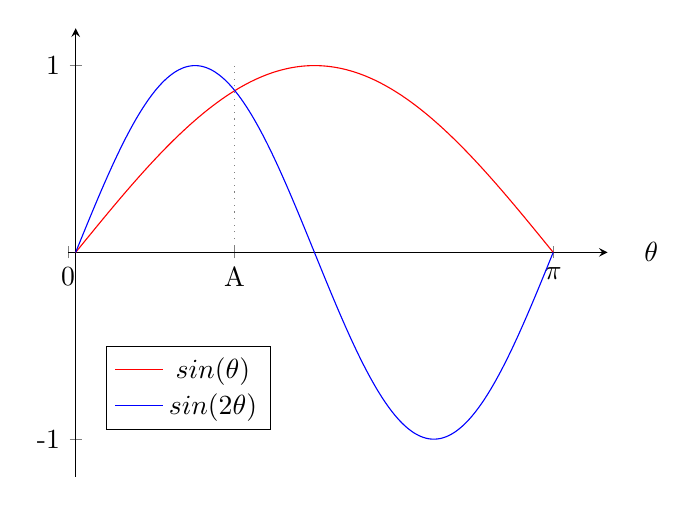
\begin{tikzpicture}\begin{axis}[axis lines=middle,samples=200
        ,xlabel=$\theta$
        ,ymax=1.2
        ,ymin=-1.2
        ,xmin = -0.05
        ,xmax = 3.5
        ,every axis x label/.style={
          at={(ticklabel* cs:1.05)},
            anchor=west,
          },
        every axis y label/.style={
          at={(ticklabel* cs:1.05)},
            anchor=south,
          },
        ,xtick=data
        ,xtick={-0.05,1.045,3.141592}
        ,xticklabels={0,A,$\pi$}
        ,ytick=data,
        ,ytick={1,-1}
        ,yticklabels={1,-1}
        ,legend style={at={(axis cs:0.2,-0.5)},anchor=north west}
        ]
      \addplot[red,domain=0:3.141592] {sin(deg(x)};
      \addplot[blue,domain=0:3.141592] {sin(deg(2*x))};
      \addplot[gray,dotted,mark=none] coordinates {(1.045, 0) (1.045, 1)};
      \legend{$sin(\theta$),$sin(2\theta$)}
\end{axis}\end{tikzpicture}
% \end{document}

	\caption{Dall'origine al punto $A$, $\Im[\P]$ ha un comportamento induttivo, tra A e $\pi$ capacitivo.}
	\label{fig:capIndutt}
\end{figure}

\section{Parametri di un'antenna}\label{sec:paramAnt}
Mostreremo ora i parametri attraverso cui un'antenna è caratterizzata, prima elencandoli e poi ricavandoli per il dipolo elementare.
I parametri, dunque, sono
\begin{itemize}
	\item Pattern di radiazione in campo e in potenza
	\item SLL - Side Lobe Level
	\item Direttività
	\item Guadagno in potenza
\end{itemize}

\subsection{Pattern di radiazione}
\paragraph{Pattern di radiazione in campo}
Si definisce \emph{pattern di radiazione in campo} il rapporto di fasori in campo lontano
\begin{equation} \label{eq:patternCampo}
	F(\theta,\phi) = \frac{E_\theta(r,\theta,\phi)}{E_\theta(r,\theta_{max},\phi_{max})}
	~ \text{ dove } ~
	\{\theta_{max} , \phi_{max}\} = \max_{\theta,\phi} |E_\theta(r,\theta,\phi)|
\end{equation}

Nel caso del dipolo elementare, si ha
\begin{esp*}
	F_{DE}(\theta,\phi)
	= \frac
		{\jmath\eta I \frac{\Delta z}{\lambda} \frac{\ejbr}{r} \sin(\theta)}
		{\jmath\eta I \frac{\Delta z}{\lambda} \frac{\ejbr}{r}}
	= \sin(\theta)
	~ \implies ~ \theta_{max}=\frac{\pi}{2}
\end{esp*}


\paragraph{Pattern di radiazione in potenza}
Definiamo il pattern di radiazione in potenza come
\begin{equation}\label{eq:patternPotenza}
	P(\theta,\phi)
	= |F(r,\theta,\phi)|^2
	= \frac
		{|E_\theta(r,\theta,\phi)|^2}
		{|E_\theta(r,\theta_{max},\phi_{max})|^2}
	= \frac{|I|}{|I_{max}|}
\end{equation}

Nel caso del dipolo elementare si ha che il pattern di radiazione in potenza è
$|F_{DE}(\theta,\phi)|^2 = \sin^2(\theta)$.

\paragraph{Solidi di direttività}
Partendo dal pattern di radiazione in campo e in potenza possiamo disegnare il \emph{solido di direttività}, un diagramma tridimensionale che permette di valutare le capacità dell'antenna in termini di emissione e radiazione.

Nel caso del dipolo elementare i suoi solidi di direttività in campo e in potenza sono visibili in figura \ref{fig:pattern}.
%TODO fare grafico, magari con CST

Poiché la maggior parte delle volte risulta difficoltoso rappresentare un grafico tridimensionale che sia facile e veloce da leggere, si decide di rappresentare un grafico bidimensionale, che verrà chiamato \emph{diagramma di radiazione}.

Il diagramma di radiazione si costruisce omettendo uno dei due angoli $\theta$ o $\phi$ e utilizzando
\begin{itemize}
	\item coordinate polari, la rappresentazione più utilizzata perché permette di cogliere immediatamente dove il campo si propaga;
	\item coordinate cartesiane, la rappresentazione che dà più risalto all'intensità del campo in determinati angoli.
\end{itemize}

\subsection{Side Lobe Level}
Dato $F_{SSL}$ il pattern del massimo di emissione del lobo secondario, il \gls{sll} si calcola come
\begin{equation}\label{eq:SLL}
	SSL=10 \, \log_{10}\left|\frac{F_{SSL}}{F_{max}}\right|^2 = 20 \, \log_{10} |F_{SSL}|
\end{equation}
dove $F_{max}=1$ per definizione.

\subsection{Direttività}
La \emph{direttività} di un'antenna quantifica la frazione di potenza emessa nel lobo (o nei lobi) principali rispetto alla potenza media irradiata.

Iniziamo quindi a determinare come la potenza emess dall'antenna in campo lontano.
\begin{equation} \label{eq:potenza_irradiata}
	P= \int_{S(r)} I(r,\theta,\phi) \de S =\int_0^\pi\int_0^{2\pi} I(r,\theta,\phi) \, r^2 \sin(\theta) \de \theta \de \phi
\end{equation}

La potenza irradiata per unità di angolo solido vale
\begin{equation*}
	U(\theta,\phi) = I(r,\theta,\phi) \, r^2
	\text{~ con ~}
	[U] = \frac{W}{sterad}
\end{equation*}

% Faremo spesso uno del suo valor massimo e valor medio, definiti come segue.
% \begin{esp*}
% 	U_m
% 	& = \max_{\theta,\phi} U(\theta,\phi)
% 	= U(\theta_{max},\phi_{max}) \\
% 	U_{AVG}
% 	& = \frac{1}{4\pi}\cdot \int U(\theta,\phi) \de \Omega
% \end{esp*}

Possiamo procedere da \autoref{eq:potenza_irradiata} con la definizione precedente.
\begin{equation}
	P = \int_0^\pi \int_0^{2\pi} U(\theta,\phi) \sin(\theta) \de \theta \de \phi
\end{equation}

Definiamo quindi la \emph{direttività} come il rapporto
\begin{esp}\label{eq:dirett}
	D
	= \frac{U_m}{U_{AVG}}
	= \frac{4\pi r^2 \, I(r, \theta_{max}, \phi_{max})}{P}
\end{esp}
dove $U_m = \max_{\theta,\phi} U(\theta,\phi)$ è il massimo e $U_{AVG} = 1/{4\pi} \int U(\theta,\phi) \de \Omega$ la media della potenza emessa per unità di angolo solido.

La quantità $4\pi r^2 I(r,\theta_{max},\phi_{max})$ viene normalmente chiamata \gls{eirp}: esso corrisponde alla potenza irradiata dall'antenna se la sua intensità in ogni direzione fosse uguale al massimo.

\paragraph{Direttività del dipolo elementare}

Sostituendo alla definizione le espressioni ricavate in precedenza per il dipolo elementare, ricaviamo che
\begin{equation*}
	\begin{dcases}
		U(\theta,\phi) = \frac{\eta |I|^2}{8} \left(\frac{\Delta z}{\lambda}\right)^2 \sin(\theta) \\
		U_m = \frac{\eta |I|^2}{8} \left(\frac{\Delta z}{\lambda}\right)^2\\
		P = \frac{\pi}{3} \, \eta |I|^2 \left(\frac{\Delta z}{\lambda}\right)^2
	\end{dcases}
	\begin{split}
		\implies ~~ D_{DE}
		& = \frac{4\pi U_m}{P}
		= \frac{\frac{\eta |I|^2}{8} \left(\frac{\Delta z}{\lambda}\right)^2 4\pi}{\frac{\pi}{3}\eta |I|^2 \left(\frac{\Delta z}{\lambda}\right)^2} \\
		& = \frac{3}{2} = 1,5
	\end{split}
\end{equation*}
Il risultato ottenuto mostra come il dipolo elementare sia poco direttivo.

\bigbreak
La direttività si può ricavare anche a partire dal pattern di radiazione $F$, in questo modo.

Prima di tutto, osserviamo che l'intensità $I$ in un punto dipende dal quadrato del modulo del campo elettrico $\E$: questo ci permette di scrivere
\begin{equation*}
	|F(\theta, \phi)|^2
	= \left|\frac{E_\theta(r, \theta, \phi)}{E_\theta(r, \theta_{max}, \phi_{max})} \right|^2
	= \frac{I(r, \theta, \phi)}{I(r, \theta_{max}, \phi_{max})}
	= \frac{U(\theta, \phi)}{U_m}
\end{equation*}

Possiamo usare questa osservazione nel calcolo di $U_{AVG}$.
\begin{equation*}
	U_{AVG}
	= \frac{1}{4\pi} \int U(\theta, \phi) \de \Omega
	= \frac{U_m}{4\pi} \int_0^\pi \int_0^{2\pi} |F(\theta, \phi)|^2  \de \phi \de \theta
	= \frac{U_m}{4\pi} \, \Omega_A
\end{equation*}
dove $\Omega_A$ è detto \emph{angolo solido del fascio}.

La direttività si può semplicemente calcolare quindi come
\begin{equation} \label{eq:def_direttivita}
	D = \frac{U_m}{U_{AVG}} = \frac{4\pi}{\Omega_A}
\end{equation}

\subsection{Guadagno in potenza}
Una qualsiasi antenna può essere vista come un generico dipolo elettrico, come in \autoref{fig:antenna_come_dipolo}.

\begin{figure}[htp]
	\centering
	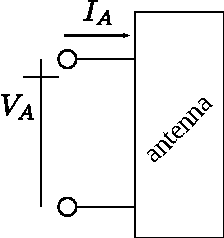
\includegraphics[]{img/antenna_come_dipolo.pdf}
	\caption{Schema elettrico di un antenna generica.}
	\label{fig:antenna_come_dipolo}
\end{figure}

Per valutare la qualità dell'antenna possiamo perciò considerare, invece della sua potenza irradiata $P$, la potenza elettrica in ingresso $P_IN$, più semplice da stabilire all'atto pratico.

Perciò definiamo il \emph{guadagno in potenza} come

\begin{equation} \label{eq:def_guadagno}
	G = \frac{4\pi \, U_m}{P_{IN}}
	\text{\quad con \quad} P_{IN} = \Re \left[ \frac{V_A \, I_A^*}{2} \right]
\end{equation}

Combinando \autoref{eq:def_guadagno} con \autoref{eq:def_direttivita}, otteniamo

\begin{equation*}
	G \cdot P_{IN} = 4\pi \, U_m = D \cdot P
	\text{\quad dove\quad} D \cdot P = EIRP = 4\pi U_m.
\end{equation*}

Siccome l'antenna è un dipolo passivo, la potenza emessa non potrà superare quella entrante, perciò la direttività è un limite superiore al valore del guadagno.
\begin{equation*}
	G = D \, \frac{P}{P_{IN}} = D\, e_r = \le D
\end{equation*}
dove $e_r$ è detta \emph{efficienza di antenna}.

\section{Impedenza d'antenna}
L'antenna, come osservato in precedenza, si comporta come un dipolo elettrico, perciò essa andrà adattata alla linea, per evitare riflessioni di potenza.

L'impedenza dell'antenna, come da \autoref{fig:antenna_come_dipolo}, vale
\begin{equation}
	Z_A = \frac{V_A}{I_A} = R_A + \jmath \Chi_A
\end{equation}
dove $R_A$ è la resistenza d'antenna e $\Chi_A$ è la reattanza d'antenna.

La potenza in ingresso si può calcolare quindi come
\begin{equation*}
	P_{IN}
	= \Re \left[ \frac{V_A \, I_A^*}{2} \right]
	= \Re \left[ \frac{Z_A \, I_A \, I_A^*}{2} \right]
	= R_A \, \frac{|I_A|^2}{2}
\end{equation*}

Essa può inoltre essere scomposta in potenza irradiata $P$ e potenza dissipata per effetto Joule $P_o$.
\begin{esp*}
	P_{IN}
	&= P + P_o
	= P + R_o \, \frac{|I_A|^2}{2}
	\stackrel{(*)}{=} R_r \frac{|I_A|^2}{2} + R_o \\
	& = \left( R_r + R_o  \right) \frac{|I_A|^2}{2}
	= R_A \, \frac{|I_A|^2}{2}
\end{esp*}
definendo $R_o$ resistenza ohmica dell'antenna e $R_r$ la \emph{resistenza di radiazione}, tale per cui $P=R_r \, |I_A|^2 / 2$.

Perciò si può esprimere l'efficienza d'antenna anche in termini di impedenza, infatti
\begin{equation*}
	e_r
	= \frac{P}{P_{IN}}
	= \frac{R_r}{R_A}
	= \frac{R_r}{R_r + R_o}
	\le 1
\end{equation*}

Nel caso del dipolo elementare, supponendo una resistenza ohmica trascurabile, otteniamo

\begin{esp}\label{eq:pot-resRadDE}
	R_r
	&= \frac{2P}{|I_A|^2}
	\stackrel{(*)}{=} \frac{2}{3}\pi \eta \left(\frac{\Delta z}{\lambda}\right)^2
	= 80\pi^2\left(\frac{\Delta z}{\lambda}\right)^2 \Omega
\end{esp}
dove in (*) si sfrutta la formula \autoref{eq:potenza_DE} della potenza irradiata dal dipolo elementare.

Poiché il rapporto $\Delta z / \lambda$ è molto piccolo, l'antenna risulta poco efficiente.

\bigbreak
Per calcolare $\Chi_A$, osserviamo ora la potenza reattiva emessa dall'antenna in campo vicino, quindi per $r \ll \lambda$.

\begin{esp} \label{eq:bilancio_EM_immaginario}
	\Im [P]
	& = \Im\left[\frac{V_A \cdot I_A^*}{2}\right]
	= \Im\left[- \int_V \E \cdot \J^* \de V\right] \\
	& \stackrel{(*)}{=}
	\omega \underbrace{\int_V \left[\mu \frac{|\H|^2}{2} - \epsilon \frac{|\E|^2}{2} \right] \de V}_{1}
	+ \underbrace{\Im\left[\int_{S(r)} \P \cdot \hat{r} \de S\right]}_{2}
\end{esp}
dove in (*) viene usata il bilancio energetico \autoref{eq:bilancio_potenza_EM_steinmetz}.

Ricordando \autoref{eq:campoEM}, proviamo ora che il termine 1 di variazione di energia elettromagnetica in \autoref{eq:bilancio_EM_immaginario} è negativo.
\begin{esp*}
	\begin{dcases}
		H_\phi \propto \frac{1}{r^2} \\
		E_\theta \propto \frac{1}{r^3}
	\end{dcases}
	\implies
	\begin{dcases}
		\frac{\mu|\H|^2}{2} \simeq \frac{\mu}{r^2} \\
		\frac{\epsilon|\E|^2}{2} \simeq \frac{\mu}{r^6}
	\end{dcases}
	\implies \frac{\epsilon|\E|^2}{2} \gg \frac{\mu|\H|^2}{2}
	\text{\quad per } r \ll \lambda
\end{esp*}

Riprendendo il calcolo \autoref{eq:campoDE_parte_imm} del vettore di Poynting per il dipolo elementare, si ha che
\begin{esp*}
	\Im[\P]
	= - \left[
		\frac{\eta}{2\beta} \, |I|^2
		\left( \frac{\Delta z}{\lambda} \right)^2
	\right]
	\, \frac{1}{r^5} \,
	\left(
		\sin^2(\theta) \hr
		- \sin(2\theta) \hth
	\right)
\end{esp*}

Il termine 2 si può calcolare quindi come
\begin{esp*}
	\Im\left[\int_{S(r)} \P \cdot \hat{r} \de S\right]
	& = \ldots
	= - \frac{\eta}{3} \, |I_A|^2 \,
	\left( \frac{\Delta z}{\lambda} \right)^2
	\left( \frac{\lambda}{2\pi r} \right)^3 \\
	& \stackrel{(*)}{\simeq} - \frac{\eta}{3} \, |I_A|^2 \,
	\left( \frac{\lambda}{r} \right)
	\frac{1}{(2\pi)^3} \ll 0
\end{esp*}
dove in (*) ci si pone in campo vicino, per cui $\Delta z \simeq r$ e $r \ll \lambda$.

Anche il termine 2 è quindi negativo, perciò dalla \autoref{eq:bilancio_EM_immaginario} anche $\Im[P]$ e $\Chi_A$ lo sono: il comportamento del dipolo in campo vicino è perciò quello di un condensatore.

\subsection{Adattamento dell'antenna}
Il segnale trasmesso da un'antenna proviene da un generatore collegato attraverso una linea (coassiale, bifilare o guida d'onda) che possiede una sua impedenza caratteristica. È quindi necessario adattare l'antenna, che considereremo come un dipolo elettrico, alla linea di trasmissione per ridurre le riflessioni e permettere che, idealmente, tutta la potenza venga trasmessa.

Definiamo quindi \emph{impedenza caratteristica della linea} la quantità
\begin{equation}
	Z_C = \frac{V_+}{I_+} = \sqrt{\frac{l}{c}}
\end{equation}

Se la linea è priva di perdite, $Z_C \in \R$ e si assume valori di 50--75$\Omega$ per linee coassiali e 100--300$\Omega$ per linee bifilari.

Definiamo ora il coefficiente di riflessione della linea.
\begin{equation}
	\rho = \frac{Z_A -Z_C}{Z_A + Z_C}
\end{equation}
dove $Z_A$ è l'impedenza d'antenna.

Nel caso del dipolo elementare sappiamo la resistenza $R_A$ è trascurabile rispetto sia alla reattanza $\Chi_A$ che ai valori di impedenza di linea indicati in precedenza.
\begin{equation*}
	|\rho|
	\simeq \frac{|\jmath \Chi_A -Z_C|}{|\jmath \Chi_A +Z_C|}
	\simeq 1
	~~ \implies ~~
	P_{IN}
	= P(1-|\rho|^2)
	= \frac{|V_+|^2}{Z_C}(1-|\rho|^2) \simeq 0
\end{equation*}

Un elevato $\rho$ rende l'antenna incapace di irradiare, perché tutta la potenza in ingresso viene riflessa al generatore.

Bisogna quindi adattare l'antenna adottando una delle seguenti strategie:
\begin{itemize}
	\item modificare $Z_A$ in modo tale che sia simile a $Z_C$. Questo è difficoltoso, perché l'impedenza d'antenna dipende principalmente dal pattern di radiazione desiderato.
	\item utilizzare adattatori d'impedenza, che però hanno due principali limiti
	\begin{itemize}
		\item introducono perdite
		\item adattano l'antenna alla linea in una banda limitata. Costruire adattatori a banda larga è più costoso e difficile da realizzare.
	\end{itemize}
\end{itemize}

% commentato perché non si capisce dove si va a parare
% TODO: sistemare

% \paragraph{Linea come quadripolo}

% Definiamo ora la matrice di scattering, una matrice quadrata di ordine $N$ che rappresenta come avviene la diffusione di un segnale che entra in un $N$-polo.

% Dato $a_i$ l'ingresso i-esimo e $b_i$ l'uscita i-esima, abbiamo
% \begin{equation}
% 	\begin{dcases}
% 		S_{ii} = \left. \frac{b_i}{a_i}\right |_{a_k = 0,~ \forall k \neq i} & \text{coefficiente di riflessione di }i \\
% 		S_{ij} = \left. \frac{b_i}{a_j}\right |_{a_k = 0,~ \forall k \neq j} & \text{coefficiente di trasmissione tra } i \text{ e } j\\
% 	\end{dcases}
% \end{equation}
% In particolare, vorremo che in un adattatore di impedenza, visto come quadripolo con due ingressi e due uscite valga $S_{ii}\to0$, in modo da evitare riflessioni.
% % da definire A e D
% \begin{esp*}
% 	P_{IN} = \frac{1}{2}
% 	\sum\limits_{i=1}^N \left( |a_i|^2 - |b_i|^2 \right)
% 	= \ldots
% 	= \frac{1}{2} A^{*^T}\cdot D \cdot A
% \end{esp*}

\section{Momento di dipolo equivalente}
Vogliamo ora cercare di estendere quanto calcolato per il dipolo elementare a qualsiasi antenna, valutando i casi in cui è possibile adottare le approssimazioni di campo lontano e, in generale, quali sono le differenze con il caso studiato in precedenza.

Ipotizziamo ora un volume delle sorgenti $V^\prime$, per cui il vettore densità totale di corrente elettrica valga
\begin{equation}
	\J(\rp) ~ \begin{cases}
		\neq 0 & \forall \rp \in V^\prime \\ 0 & \text{altrove}
	\end{cases}
\end{equation}

Andiamo ora a valutare il potenziale vettore magnetico $\A$ per un generico punto $P$ nello spazio, individuato come in \autoref{fig:momento_equivalente}.

\begin{figure}[htp]
	\centering
	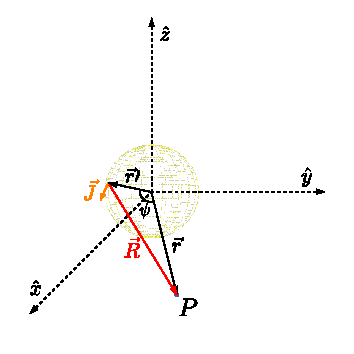
\includegraphics[]{img/momento_equivalente.pdf}
	\caption{Ciascuna sorgente $\J$ del volume $V^\prime$ delle sorgenti irradia su $P$.}
	\label{fig:momento_equivalente}
\end{figure}

Il contributo della sorgente infinitesima $\J$ al potenziale vettore magnetco vale
\begin{equation}
	\de \A(\r)
	= \frac{\mu}{4\pi} \J(\rp) \, \frac{e^{-\jmath \beta R}}{R} \de \rp
\end{equation}

Il potenziale effettivo su $P$ risulta perciò
\begin{equation} \label{eq:A_di_P}
	\A(\r)=\int_{V^\prime} \de \A(\rp) =\int_{V^\prime} \frac{\mu}{4\pi} \J(\rp) \frac{\ejbr}{R} \de \rp
\end{equation}

Come si può notare in \autoref{fig:momento_equivalente}, la distanza $R$ di $P$ dalla sorgente dipende sia da $r$, $r^\prime$ e $\phi$, secondo il teorema del coseno.

Cerchiamo quindi un'approssimazione per il calcolo di $R$ che ci faciliti i calcoli successivi.

\begin{esp} \label{eq:approssimazione_per_R}
	R&
	= |\r - \rp|
	= \sqrt{r^2 -2 r \, r^\prime \cos(\psi) + {r^\prime}^2} \\
	&= r \, \sqrt{1 - 2\cos(\psi) \left( \frac{r^\prime}{r}\right) + \left(\frac{r^\prime}{r}\right)^2} \\
	&\stackrel{(1)}{\simeq} r \, \sqrt{1 - 2\cos(\psi) \left( \frac{r^\prime}{r}\right) + o\left(\frac{r^\prime}{r}\right)} \\
	&\stackrel{(2)}{\simeq} r \left[ 1 - \cos(\psi) \left( \frac{r^\prime}{r}\right) + o\left(\frac{r^\prime}{r}\right) \right]
\end{esp}
dove in (1) viene aggiunta alle ipotesi di campo lontano $r \gg \rp$, mentre in (2) viene impiegato il limite notevole $\sqrt{1 + x} \simeq 1 + x/2$ per $x \to 0$.

Riprendendo \autoref{eq:A_di_P}, possiamo quindi scrivere
\begin{equation} \label{eq:A_generico}
	\A(\r)
	\simeq \int_{V^\prime} \frac{\mu}{4\pi} \J(\rp) \, \frac{e^{-\jmath\beta \, [r-r^\prime cos(\psi)]}}{r} \de \rp
\end{equation}
dove il denominatore viene approssimato a $r$ date le condizioni di campo lontano impostate in precendenza.
Al numeratore rimane il termine al grado 1, perché $\beta \, r^\prime = 2\pi r^\prime / \lambda$ non necessariamente risulta trascurabile come termine di fase.

Riorganizzando i termini, si può arrivare ad un espressione analoga a quella del dipolo elementare, reperibile in \autoref{eq:A_DE}.

\begin{esp*}
	\A(\r)
	&=
	\frac{\mu\ejbr}{4\pi r}
	\int_{V^\prime}\J(\rp)\, e^{-\jmath\beta r^\prime cos(\psi)} \de \rp \\
	&=\frac{\mu \ejbr}{4\pi r} \M(\theta,\phi)\\
\end{esp*}
dove $\M(\theta,\phi)$ è detto \emph{momento di dipolo equivalente}.
Nel caso del dipolo elementare vale semplicemente $I \Delta z \hhat{z}$.

Questa espressione vale solamente se reggono le approssimazioni utilizzate in precedenza, ricapitolando

\begin{equation} \label{eq:campo_lontano_generico}
	\begin{dcases}
		r \gg \lambda \\
		r \gg r^\prime \quad \forall r^\prime \in V^\prime \\
		\beta \frac{(r^\prime)^2}{r}
		= \frac{2\pi}{\lambda} \frac{(r^\prime)^2}{r}
		\le \frac{2\pi D^2}{\lambda r}
		\ll 1
		~~ \implies ~~
		r \gg \frac{2\pi D^2}{\lambda}
	\end{dcases}
\end{equation}
dove $D \ge \max_{V^\prime} r$ è la grandezza dell'antenna.

L'ultima condizione è necessaria affinché il termine quadratico in $r^\prime$ in \autoref{eq:A_generico} risulti effettivamente trascurabile nel termine di fase.

\subsection{Altezza efficace}
Definiamo l'\emph{altezza efficace in trasmissione} come il termine $\h_T(\theta,\phi)$ tale per cui
\begin{equation}
	\E
	= \jmath \frac{\eta}{2\lambda} \frac{\ejbr}{r} \, \h_T(\theta,\phi) \, I_A
\end{equation}
dove $I_A$ è la corrente ai morsetti dell'antenna.

Nel caso del dipolo elementare si ha che $\h_T(\theta,\phi) = \Delta z \hz$.

\bigbreak
Consideramo ora il caso reciproco, quello della \emph{ricezione}, prendendo come riferimento lo schema in \autoref{fig:altezza_efficace}.

\begin{figure}[htp]
	\centering
	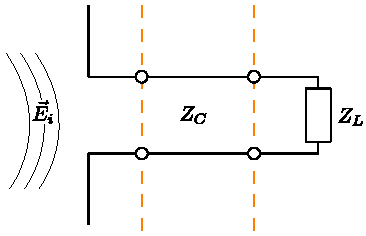
\includegraphics[]{img/altezza_efficace.pdf}
	\caption{Schema elettrico della ricezione di un segnale.}
	\label{fig:altezza_efficace}
\end{figure}

Supponiamo il carico sia adattato, quindi  $Z_L=Z_C$, e definiamo $\E_i$ come il campo elettrico incidente sull'antenna determinato in assenza dell'antenna stessa.

Per il teorema di Thevenin, esiste un generatore equivalente all'antenna, di tensione a vuoto $V_G$ e impedenza $Z_G$.

Definiamo $\h_R$ l'\emph{altezza efficace in ricezione} come il termine per cui la tensione a vuoto dell'antenna vale
\begin{equation}
	V_G=\E_i \cdot \h_R^*(\theta,\phi)
\end{equation}

La potenza al ricevitore sarà quindi
\begin{esp*}
	P_{RX}
	& = \Re\left[\frac{V_L \, I_L^*}{2}\right]
	= \frac{|V_G|^2}{2} \frac{R_L}{|Z_L+Z_G|^2}
	= \frac{R_L \, |\E_i \cdot \h_R^*|^2}{2 \, |Z_L+Z_G|^2} \\
	& \stackrel{(*)}{=} \frac{R_L \, |\E_i \cdot \h_R^*|^2}{2 \, |Z_L+Z_A|^2}
\end{esp*}
dove (*) vale per il teorema di reciprocità.

Si può osservare come una corretta disposizione dei vettori campo elettrico e antezza efficace sia indispensabile per una buona ricezione, per questo motivo definiamo l'\emph{adattamento di polarizzazione}.

\begin{equation}
	p
	=\frac{|\E_i \cdot \h_R^*|^2}{|\E_i|^2 |\h_R|^2}
	= \left|
		\frac{\E_i}{|\E_i|}\cdot\frac{\h_R}{|\h_R|}
	\right|^2
	= |\hat{e}_i \cdot \hat{h}_R^*|^2
\end{equation}
in cui $\hat{e}_i$ e $\hat{h}_R^*$ sono i fasori di direzione dei corrispondenti vettori.

Nel caso di vettori complessi a polarizzazione ortogonale, $p$ si riduce a 0, così come la potenza ricevuta.
\begin{equation}
	\E_i \cdot \h_R^* =0 \Leftrightarrow \E_i \perp \h_R
\end{equation}

Nel caso invece i due vettori siano paralleli, $p = 1$ e la potenza ricevuta è massima.
\begin{equation}
	\E_i \cdot \h_R^* = \gamma |\h_R|
	\Leftrightarrow \E_i \parallel \h_R
	\Leftrightarrow p=1
\end{equation}

\bigbreak
Inoltre, per il teorema di reciprocità, si può affermare che le due differenti definizioni di altezza efficace coincidono.
\begin{equation}
	\h_T(\theta,\phi) = \h_R(\theta,\phi)
\end{equation}

\paragraph{Esempio GNSS}
Nel caso di navigazione satellitare, sistemi come il GPS, il \textsc{GLONASS}, Beidou e \textsc{IRNSS} utilizzano una polarizzazione circolare destrorsa, in quanto l'onda, dopo una riflessione, inverte il verso di polarizzazione e si attenua.

L'antenna del cellulare, quindi, filtra naturalmente una riflessione. In caso di doppia riflessione su materiale non conduttore il segnale è molto più attenuato, per cui verrà considerato come rumore di fondo, mentre persiste nel caso del buon conduttore.

Le espressioni dei campi incidente e riflesso sono qui riportate.
\begin{esp*}
	\E_i &= (E_x \cdot \hat{x}+E_y \cdot \hat{y}) \cdot e^{\textcolor[rgb]{0.8,0,0}{-}\jmath \beta z} \\
	\E_r &= (E_x \cdot \hat{x}+E_y \cdot \hat{y}) \cdot \rho \cdot e^{\textcolor[rgb]{0.8,0,0}{+}\jmath \beta z} \\
\end{esp*}

\subsection{Area efficace}
Definiamo area efficace di un'antenna il rapporto:
\begin{equation}\label{eq:Aeff}
	A_{em}=\frac{P_{R,\, max}}{I_i(r,\theta,\phi)} \quad [A_{em}] = m^2
\end{equation}

dove $I_i(r,\theta,\phi)$ è l'intensità di radiazione nel punto dove si pone l'antenna, in assenza dell'antenna stessa.

% Supponiamo che il carico sia adattato, quindi che $Z_L = Z_A^*$: in questo caso la potenza ricevuta è massima e si può scrivere
% \begin{equation*}
% 	A_{em}
% 	= \frac{|\E_i|^2 \, |\h_{R, max}|^2}{8 R_A} \, \frac{2\eta}{|E_i|^2}
% 	= \frac{\eta}{4 R_A} \, |\h_{R, max}|^2
% \end{equation*}

\subsection{Ottimizzazione della potenza ricevuta}
La potenza ricevuta dipende da molteplici parametri del ponte radio: per avere un segnale ottimale è necessario che ci sia

\begin{enumerate}
	\item adattamento del carico \hfill $Z_L = Z_A^*$
	\item adattamento in polarizzazione \hfill  $p = 1$
	\item corretto orientamento dell'antenna ricevente \hfill $\h_R = \h_{R,\, max}$
\end{enumerate}

Sotto queste condizioni, si può calcolare l'area efficace massima come
\begin{equation*}
	A_{em}
	= \frac{|\E_i|^2 \, |\h_{R, max}|^2}{8 R_A} \, \frac{2\eta}{|E_i|^2}
	= \frac{\eta}{4 R_A} \, |\h_{R, max}|^2
\end{equation*}

Nel caso del dipolo elementare, osserviamo che l'area efficace \emph{non} dipende dalla lunghezza $\Delta z$, ma solamente dalla lunghezza d'onda.
\begin{equation*}
	A_{em}
	= \frac{\eta}{4 R_A} \, |\h_{R, max}|^2
	= \frac{\eta}{4 R_A} \, {\Delta z}^2
	= \frac{\eta}{4 \left(
			\frac{2}{3} \pi \eta \left(
				\frac{\Delta z}{\lambda}
			\right)^2
		\right)} \, {\Delta z}^2
	= \frac{3 \lambda^2}{8\pi}
\end{equation*}

\subsection{Parametri di antenna in TX e RX}

I parametri in ricezione definiti finora risultano slegati da quelli in trasmissione: il teorema di reciprocità suggerisce tuttavia una forte relazione gli uni con gli altri.

Ricaviamo ora il modulo del campo elettrico massimo rispettivamente in trasmissione e in ricezione, per poter applicare il suddetto teorema.

\begin{esp}
	4\pi\, U_m &= D \, P \\
	4\pi r^2 \, I(r,\theta_{max},\phi_{max}) &= D \, P_{tx} \\
	4\pi r^2 \, \frac{|\E_{tx,\, max}|^2}{2\eta} &= D \, \frac{R_r \, |I_A|^2}{2} \\
	|\E_{tx,\, max}|^2 &=
	\eta \, D \, \frac{R_r \, |I_A|^2}{4\pi r^2}
\end{esp}

\begin{esp}
	|\E_{i,\, max}|^2
	= \max \left|
		\jmath\, \frac{\eta}{2\lambda}\, \frac{\ejbr}{r} \,
		\h_R \, I_A
	\right|^2
	= \left[
		\frac{\eta \, |\h_{R,\,max}| \, |I_A|}{2\lambda r}
	\right]^2
\end{esp}

Combinando le due equazioni per il campo elettrico, troviamo che

\begin{esp} \label{eq:rapportoParam}
 \left[
		\frac{\eta \, |\h_{R,\,max}| \, |I_A|}{2\lambda r}
	\right]^2
	&= \eta \, D \, \frac{R_r \, |I_A|^2}{4\pi r^2} \\
	\frac{\eta \, |\h_{R,\,max}|^2}{4 R_A} \,
	\frac{1}{\lambda^2}
	&= \frac{D}{4\pi} \, \frac{R_r}{R_A} \\
	\frac{A_{em}}{D} &= \frac{\lambda^2}{4\pi}
\end{esp}
dove nel primo passaggio si è diviso a destra e a sinistra per $4R_A$, mentre nel secondo si è sfruttato il legame tra area efficace massima e altezza efficace massima.
Inoltre si è supposta un'antenna senza perdite, dove quindi $R_r = R_A$.

Verifichiamo ora la relazione appena ricavato nel caso del dipolo elementare.
\begin{esp*}
	\begin{dcases}
		D =\frac{3}{2} \\
		A_{e,\,max}=\frac{3}{8\pi}\, \lambda^2
	\end{dcases}
	~~ \implies ~~
	\frac{A_{e,\,max}}{D} =\frac{\frac{3}{8\pi}\, \lambda^2}{\frac{3}{2}} = \frac{\lambda^2}{4\pi}
\end{esp*}

Le antenne reali presentano però delle perdite: l'utile proprietà appena ricavata si può estendere al caso generale in questo modo.
\begin{equation*}
	\frac{A_{em}}{D} \, \frac{e_r}{e_r}
	= \frac{\lambda^2}{4\pi}
	~~ \implies ~~
	\frac{A_{e}}{G}
	= \frac{\lambda^2}{4\pi}
\end{equation*}

\section{Formula di Friis}
La formula di Friis permette di stabilire la potenza al ricevitore in un ponte radio, per esempio quello descritto in \autoref{fig:due_antenne_adattamento}.

\begin{figure}[htp]
	\centering
	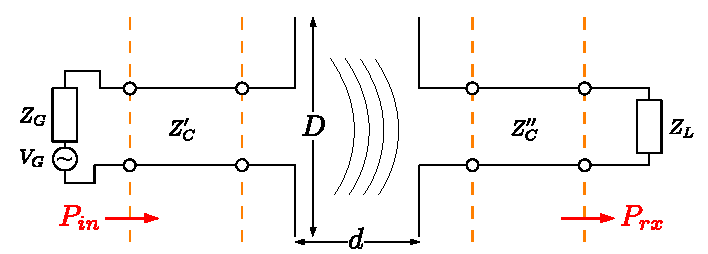
\includegraphics[]{img/due_antenne_adattamento.pdf}
	\caption{Esempio completo di collegamento radio.}
	\label{fig:due_antenne_adattamento}
\end{figure}

Il suo utilizzo richiede che siano verificate le seguenti condizioni:
\begin{enumerate}
	\item le antenne sono in campo lontano l'una rispetto all'altra
	\begin{equation*}\begin{dcases}
		d\gg \lambda & \text{se } D \ll \lambda \\
		d \gg \frac{2D^2}{\lambda} & \text{se } D\ge 2,5\lambda
	\end{dcases}\end{equation*}
	\item adattamento dei carichi in trasmissione e ricezione, sia alla linea che alle antenne
	\item adattamento in polarizzazione dell'antenna ricevente
	\item orientamento ottimale tra le due antenne
\end{enumerate}

Sotto queste condizioni possiamo ricavare la potenza ricevuta, con le proprietà ricavate in precedenza.
\begin{esp*}
	EIRP&= G_{TX}\, P_{IN}\\
	\frac{|\E_{i_{max}}|^2}{2\eta}\, 4\pi d^2 &= G_{TX}\, P_{IN} \\
	\frac{|\E_{i,\,max}|^2}{2\eta} &= \frac{G_{TX}\, P_{IN}}{4\pi d^2}\\
	P_{R, \,max} &= \frac{|\E_{i,\,max}|^2}{2\eta} \, A_{e, \, max}^{RX} = \frac{G_{TX}\, P_{IN}}{4\pi d^2}\, \frac{\lambda^2}{4\pi}\, G_{RX}
\end{esp*}

Si ottiene infine la \emph{formula di Friis}.
\begin{equation}\label{eq:friis}
	P_{R,\,max}
	= G_{TX}\, G_{RX}\, P_{IN} \left(\frac{\lambda}{4\pi d}\right)^2
\end{equation}

%%% Local Variables:
%%% mode: latex
%%% TeX-master: "antenne"
%%% End:
